\documentclass[11pt,letterpaper]{article}
\PassOptionsToPackage{hyphens}{url}
\usepackage[margin=.83in,top=.8in,bottom=.8in,headheight=15pt]{geometry}
\usepackage[T1]{fontenc}
\usepackage{lmodern,amsmath,amssymb,mathtools,bm,booktabs,array,graphicx,tikz}
\usetikzlibrary{arrows.meta,positioning,calc,decorations.pathreplacing,patterns}
\definecolor{ink}{HTML}{17344D}\definecolor{accent}{HTML}{087E8B}\definecolor{pale}{HTML}{EDF5F5}\definecolor{gold}{HTML}{AD6B19}
\providecommand{\dd}{\,\mathrm{d}}\providecommand{\R}{\mathbb{R}}
\providecommand{\E}{\mathbb{E}}\providecommand{\Var}{\operatorname{Var}}
\providecommand{\Cov}{\operatorname{Cov}}\providecommand{\diag}{\operatorname{diag}}
\providecommand{\norm}[1]{\left\lVert#1\right\rVert}
\providecommand{\abs}[1]{\left|#1\right|}
\usepackage{microtype,hyperref,fancyhdr,enumitem,amsthm,sectsty,needspace}
\allsectionsfont{\raggedright}
\hypersetup{colorlinks=true,linkcolor=ink,urlcolor=accent,pdfauthor={Zan Ahmad},pdftitle={Heat-flow operators, generators and finite spectral families / Lecture notes}}
\setlength{\parindent}{0pt}\setlength{\parskip}{6pt}\linespread{1.07}
\setlist{itemsep=3pt,topsep=4pt,leftmargin=*}
\emergencystretch=2em\clubpenalty=10000\widowpenalty=10000
\pagestyle{fancy}\fancyhf{}\fancyhead[L]{\small Computational Cardiology}\fancyhead[R]{\small Lecture 17}
\fancyfoot[L]{\footnotesize Zan Ahmad}\fancyfoot[R]{\footnotesize\thepage}\renewcommand{\headrulewidth}{.3pt}
\newtheorem{proposition}{Proposition}\newtheorem{theorem}{Theorem}\newtheorem{lemma}{Lemma}
\theoremstyle{definition}\newtheorem{definition}{Definition}\newtheorem{example}{Example}
\numberwithin{equation}{section}
\begin{document}
{\small\scshape Computational Cardiology\hfill Lecture 17}\par\medskip
{\raggedright\hyphenpenalty=10000\exhyphenpenalty=10000\LARGE\bfseries\color{ink} Heat-flow operators, generators and finite spectral families\par}\medskip
{\small Lecture notes}\par\bigskip
A function-to-function map is distinct from the array used to represent it. The sealed heat equation supplies an exact example: its generator is a differential operator, its flow attenuates cosine coefficients, and its observations select particular features of the resulting field. The distinction determines both the surrogate target and the cases that must remain separate during evaluation.

\section{Functions, sampled fields and input families}
\hypertarget{note-functions-sampled-fields-and-input-families}{}\label{note:functions-sampled-fields-and-input-families}
{\small \href{slides.html\#frame=a-function-and-its-representation-panel-1\&step=1}{Slides for this section}}\par
A function assigns a value to every position in its domain. A computer stores samples or coefficients of that function. If the mesh changes from sixty-four to one hundred twenty-eight points, the stored vector changes dimension, although the underlying physical field and question may be unchanged. A finite-vector predictor can be useful on one prescribed mesh. An operator-learning objective asks for a rule between functions, together with a numerical representation that approximates that rule across specified discretizations. Calling a network an operator does not by itself prove resolution transfer.

We use a sealed one-dimensional heat equation as a transparent benchmark. Space, time and field amplitude are nondimensional, the interval is fixed, and diffusivity is spatially constant. The input is an initial field, with diffusivity supplied as a parameter when that parameter is allowed to vary. The output may be a field at one time, an entire trajectory, or a scalar such as its mean. Those are different prediction problems. The exact solution is inexpensive here, so the example is designed to reveal assumptions rather than motivate replacing this particular solver with machine learning.

A complete problem statement specifies the domain, boundary conditions, admissible inputs, parameter ranges, output horizon and error norm. Without those details, a good-looking prediction cannot be assigned a clear scope. The notebook begins with one field evolving over time, then changes diffusivity while holding the same initial field fixed.

Write $\mathcal F_K=\operatorname{span}\{1,\cos(\pi x/L),\ldots,\cos(K\pi x/L)\}$. Sampling a member of $\mathcal F_K$ on a resolved grid embeds a $(K+1)$-dimensional function family into a longer vector. Increasing the number of samples changes that embedding, not the intrinsic number of coefficients in the family.
\begin{center}\begin{minipage}{.98\linewidth}\centering
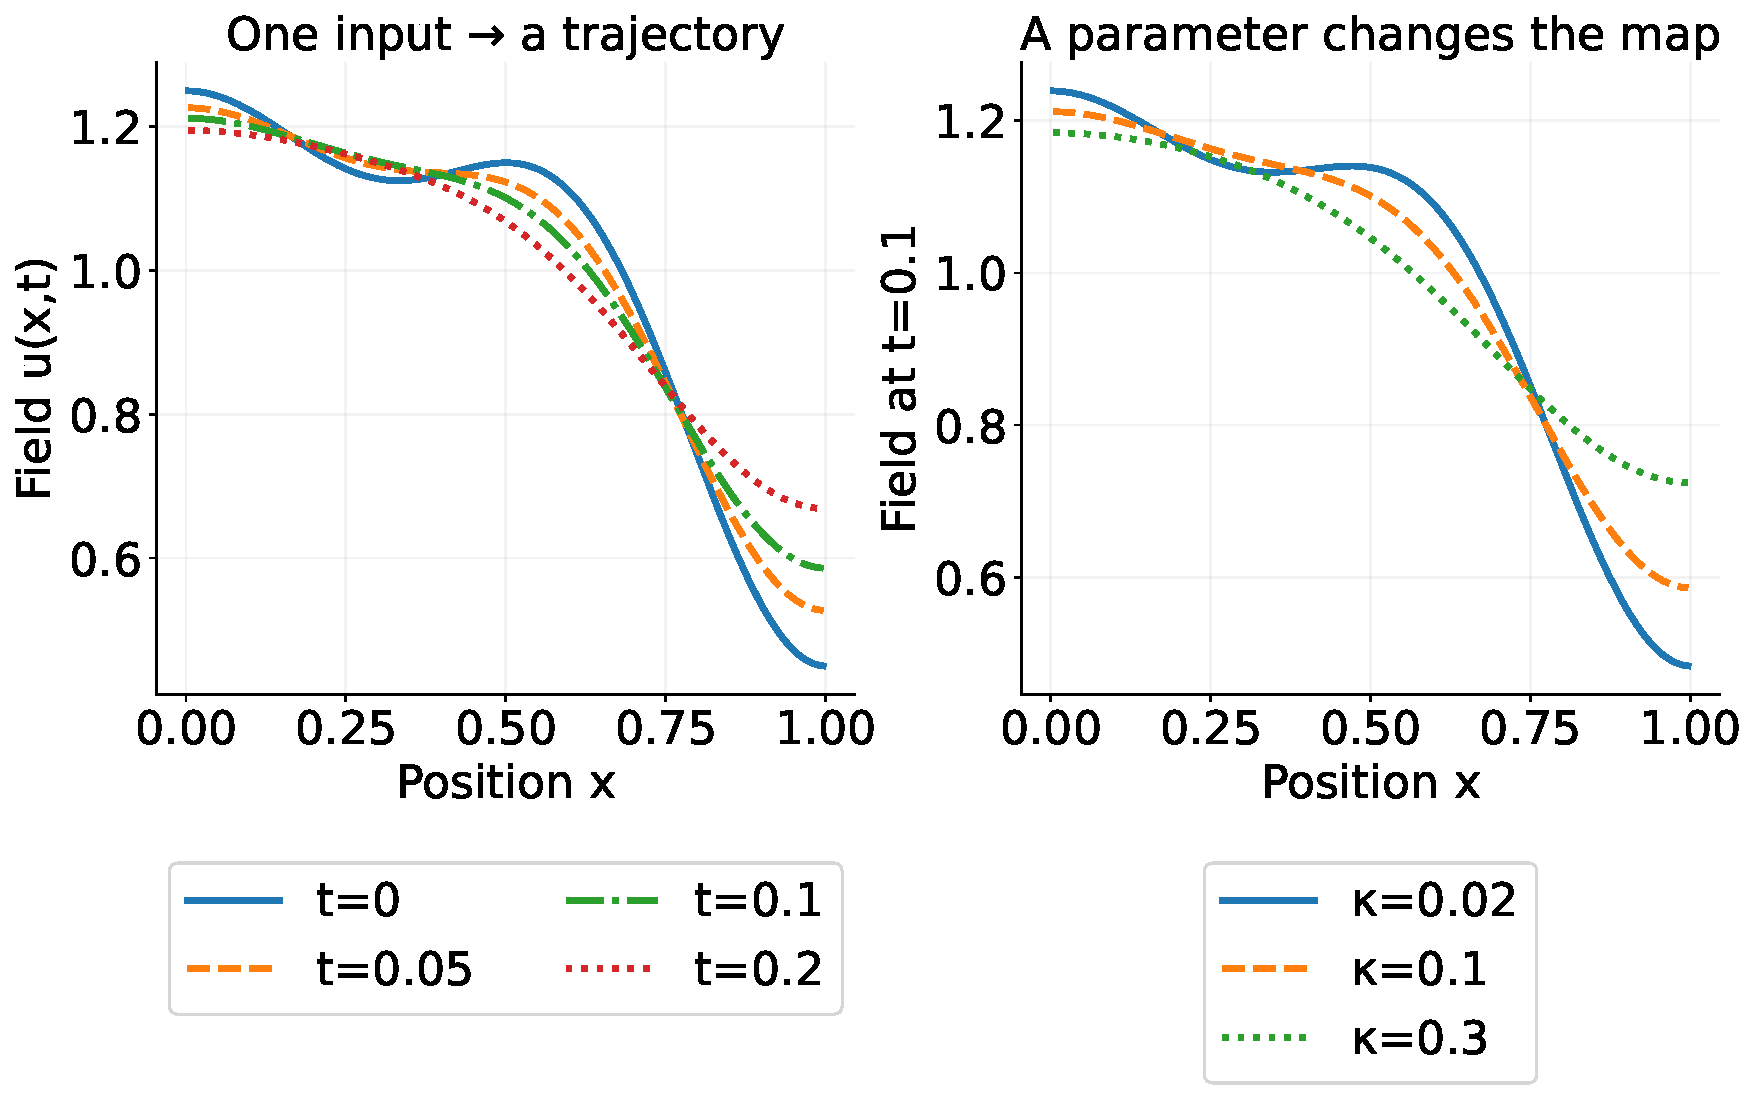
\includegraphics[width=.96\linewidth,height=.57\textheight,keepaspectratio]{operator-family.pdf}\par\smallskip
{\small Original exact sealed-heat fields. The left panel varies time for one input; the right varies diffusivity at fixed time. All scales are nondimensional.}
\end{minipage}\end{center}
\section{The Neumann heat solution by cosine expansion}
\hypertarget{note-the-neumann-heat-solution-by-cosine-expansion}{}\label{note:the-neumann-heat-solution-by-cosine-expansion}
{\small \href{slides.html\#frame=the-sealed-heat-equation\&step=1}{Slides for this section}}\par
The sealed boundary condition requires a zero spatial derivative at both ends. Cosine modes satisfy that condition: differentiating a cosine produces a sine that vanishes at each endpoint. Substituting one cosine into the heat equation gives a scalar decay equation for its amplitude. Mode k decays at rate diffusivity times the square of k\ensuremath{\pi}/L. A constant field is the zero-frequency mode and does not decay. Because this PDE is linear, a finite sum of these modes evolves by decaying each amplitude separately.

This gives a function-to-function map without any training. At a chosen final time, multiply each nonconstant input coefficient by its known attenuation and reconstruct the field. A trajectory is the family of such outputs as time varies. Higher modes decay faster, which smooths the field while preserving its mean. The mean alone cannot describe that smoothing: many distinct profiles share exactly the same average.

The companion samples the continuous formula at cell midpoints and uses only modes well below the grid limit. For these resolved cosine modes, equal-weight midpoint sums recover the mean and mode coefficients to roundoff. This exact finite-family quadrature is a property of the chosen basis and grid, not a guarantee for arbitrary rough functions or irregular meshes. The explicit family makes it possible to separate a representation limitation from a coding defect.

\[
\partial_t u=\kappa\partial_{xx}u,\quad\partial_xu(0,t)=\partial_xu(L,t)=0
\]
All quantities are nondimensional in the teaching fixture.

\[
u(x,t)=a_0+\sum_{k=1}^K a_k e^{-\kappa(k\pi/L)^2t}\cos(k\pi x/L)
\]
K is a stated finite input bandwidth, not a learned universal function space.

Substituting $u(x,t)=a_k(t)\cos(k\pi x/L)$ gives
\[
 \dot a_k=-\kappa(k\pi/L)^2a_k,
 \qquad a_k(t)=e^{-\kappa(k\pi/L)^2t}a_k(0).
\]
The $k=0$ equation is $\dot a_0=0$. Orthogonality also yields
\[
 \int_0^L|u(x,t)-a_0|^2\,\mathrm dx
 =\frac L2\sum_{k\ge1}|a_k(0)|^2e^{-2\kappa(k\pi/L)^2t},
\]
so every nonconstant resolved mode decays while the mean is preserved.

\paragraph{Calculation.} Use L=1, kappa=0.1 and initial field 1+0.2 cos(\ensuremath{\pi}x). Find the output at time 0.1.

The first-mode gain is exp(\ensuremath{-}0.01\ensuremath{\pi}\ensuremath{^{2}})=0.9060181.

The new amplitude is 0.2\ensuremath{\times}0.9060181=0.1812036.

The output is 1+0.1812036 cos(\ensuremath{\pi}x), with mean 1 and endpoint values about 1.181204 and 0.818796.

The function changes while the same analytic rule can be sampled on many grids.
\section{Generator, flow and observation maps}
\hypertarget{note-generator-flow-and-observation-maps}{}\label{note:generator-flow-and-observation-maps}
{\small \href{slides.html\#frame=the-generator\&step=1}{Slides for this section}}\par
The generator maps a current state to its instantaneous time derivative. For this heat equation it is the differential operator kappa times the second derivative. The flow map advances a full field by a specified elapsed time. It is obtained by integrating the generator. A fixed-time solution operator is one member of that family of flow maps. A scalar observable, such as the spatial mean or a threshold-arrival time, is another map applied to the field or trajectory afterward.

This distinction matters for the GFuNK reading. The verified paper describes learning a generator in a graph spectral representation and numerically integrating it to obtain trajectories. That is more than fitting a direct fixed-time input/output table. The paper also notes that, when hidden ionic variables are omitted, a learned voltage-only evolution is an effective closure over its training distribution rather than a globally valid autonomous model of every ionic state. Our elementary heat equation has no such hidden variables.

For an exact autonomous flow, advancing by one interval and then another equals advancing by their sum. The code checks this semigroup identity using analytic cosine coefficients. A numerical time step or learned map may violate the identity, or may satisfy it only on a restricted family. State which map is being tested before interpreting the result. A correct mean prediction alone cannot establish that the full flow or generator has been recovered.

\[
\mathcal N_\kappa[u]=\kappa u_{xx},\quad\Phi_t^\kappa[u_0]=u(\cdot,t),\quad\Phi_s^\kappa\circ\Phi_t^\kappa=\Phi_{s+t}^\kappa
\]
The semigroup statement assumes the same equation, domain, boundary conditions and diffusivity.

Denote the generator by $\mathcal A_\kappa=\kappa\partial_{xx}$ with its stated Neumann boundary domain. The flow is $\Phi_t^\kappa=e^{t\mathcal A_\kappa}$, and an observable such as the mean is $\mathcal M[u]=L^{-1}\int_0^Lu\,\mathrm dx$. The identities
\[
 \Phi_s^\kappa\Phi_t^\kappa=\Phi_{s+t}^\kappa,
 \qquad\mathcal M[\Phi_t^\kappa u]=\mathcal M[u]
\]
express different properties. Mean preservation alone leaves every nonconstant mode undetermined.
\section{Complete-case data partitions}
\hypertarget{note-complete-case-data-partitions}{}\label{note:complete-case-data-partitions}
{\small \href{slides.html\#frame=split-complete-evolution-cases-panel-1\&step=1}{Slides for this section}}\par
A trajectory contains strongly related observations. Neighboring spatial samples share the same initial condition, and successive snapshots belong to the same evolution. Randomly splitting those individual numbers can put nearly identical information in training and test sets. The resulting test error answers a much easier interpolation question than prediction for a new initial condition. The unit assigned to a split is a complete case: its input coefficients, initial field and all output snapshots.

The deterministic dataset draws a mean and three cosine amplitudes from stated intervals. Forty-eight cases form the training regime and sixteen separately seeded cases form a held-out regime. The identifier sets are disjoint. Separate seeds help make the example reproducible, but the essential protection is the grouping rule, not the seed itself. A real geometry study might need grouping by anatomy, subject or simulation family rather than by snapshot.

A dataset card records input bandwidth, coefficient ranges, diffusivity, domain length, time horizon, grid, case count, random seed and reference method. It also names what is excluded. Our same-regime test uses new coefficients in the same three-mode family. It does not test a fourth input mode, another diffusivity, another boundary condition or a changed geometry. Those should be deliberate additional regimes, with their own labels and interpretation.

A case consists of its coefficient vector, physical parameters and entire output trajectory. Splitting cases retains the dependence among snapshots rather than treating those snapshots as unrelated examples. Holding out new coefficients in $\mathcal F_3$ tests interpolation within that family; holding out a new diffusivity, domain or input mode changes the mathematical operator problem.
\begin{center}\begin{minipage}{.98\linewidth}\centering
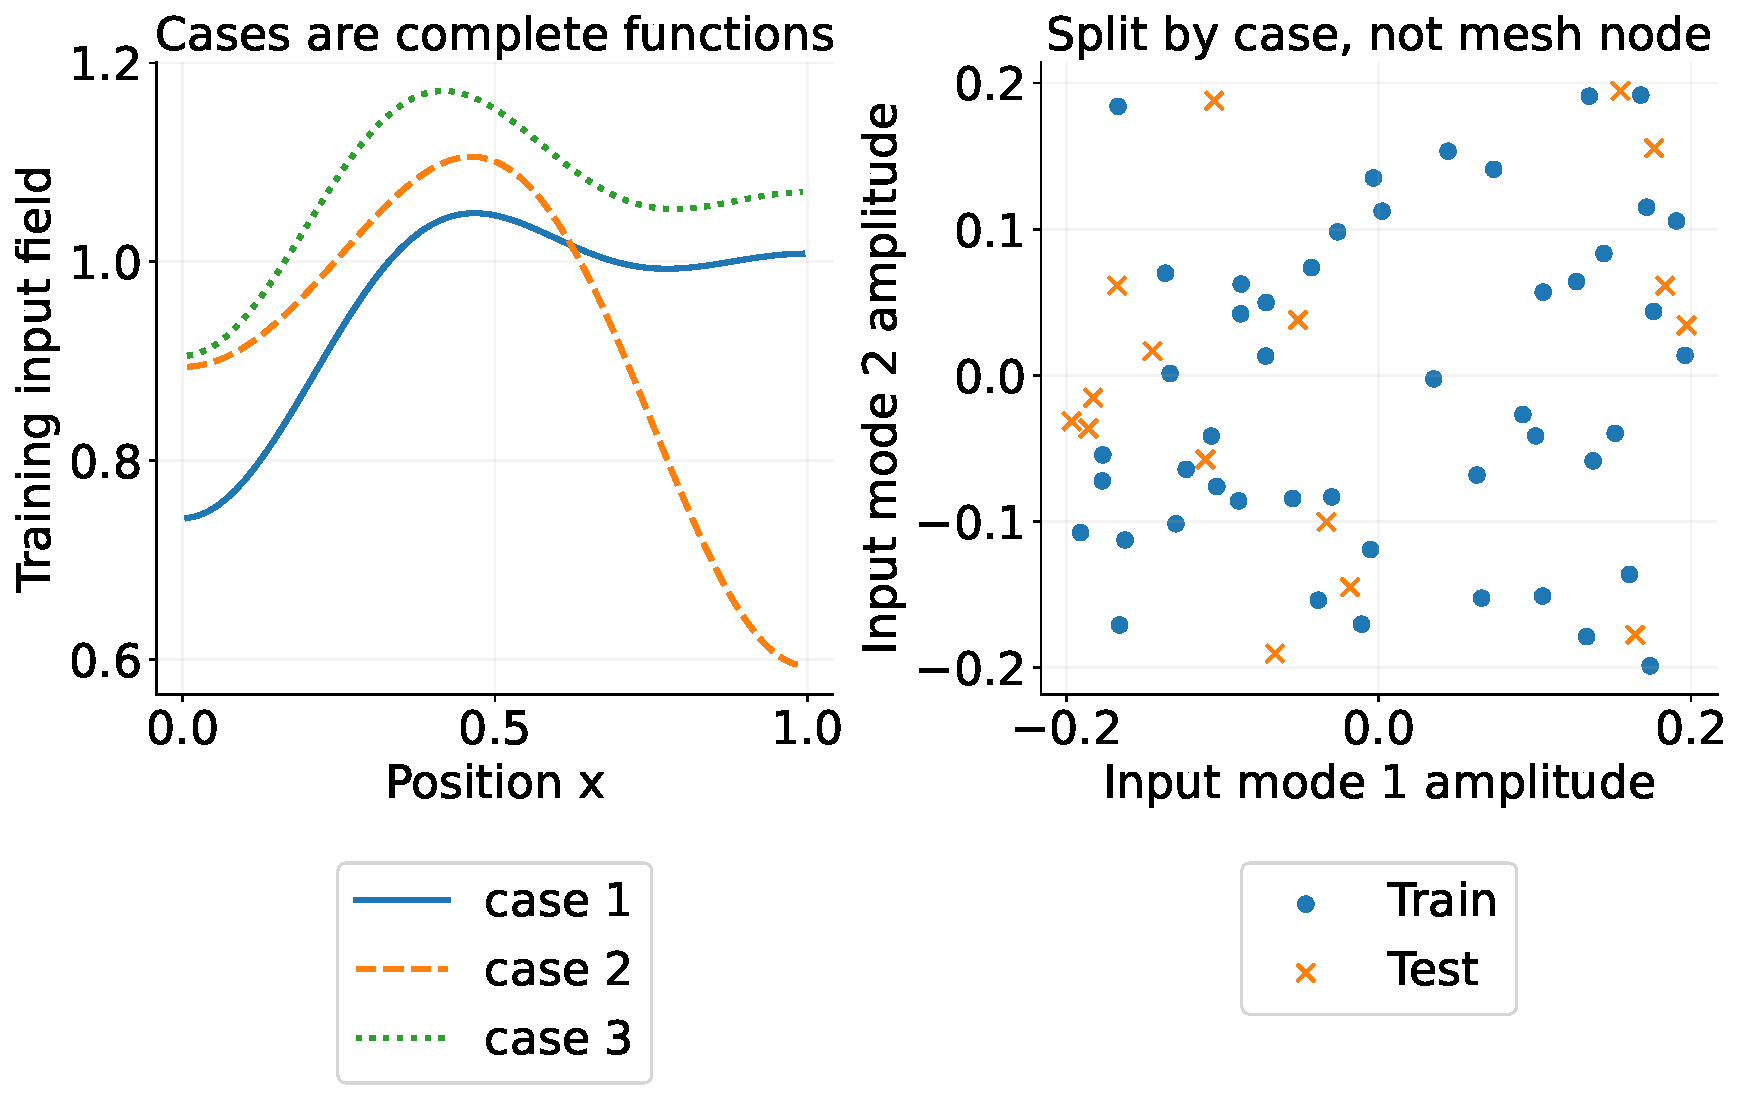
\includegraphics[width=.96\linewidth,height=.57\textheight,keepaspectratio]{dataset-regimes.pdf}\par\smallskip
{\small Original deterministic synthetic data. Complete initial conditions and their outputs stay together; a two-coefficient projection shows the regimes but does not display the full input space.}
\end{minipage}\end{center}
\section{Discrete diffusion and independent reference solutions}
\hypertarget{note-discrete-diffusion-and-independent-reference-solutions}{}\label{note:discrete-diffusion-and-independent-reference-solutions}
{\small \href{slides.html\#frame=the-discrete-cosine-decay-rate\&step=1}{Slides for this section}}\par
A synthetic label is only as reliable as the method that produced it. Here the analytic expression provides a reference independent of the numerical heat solver. The finite-volume solver uses shared neighboring fluxes and sealed endpoints. Backward Euler advances the resulting linear system. The code checks that a constant remains constant and that the discrete diffusion matrix gives the expected evolution of a cosine eigenmode. These tests examine the implementation rather than merely comparing it with data generated by itself.

For a separate spatial test, we evolve the discrete cosine mode exactly in time using its discrete eigenvalue. Comparing this semi-discrete solution with the continuous cosine formula removes time-step error from the experiment. The observed spatial error is approximately second order for this smooth resolved family. A small dense matrix exponential independently checks the discrete eigenvalue construction. None of these claims automatically extends to discontinuous inputs, irregular grids or nonlinear cardiac waves.

The useful output is an evidence chain: stated PDE, analytic derivation, sampling rule, independent component test and a recorded error measure. A three-gain spectral surrogate exactly represents a small subset of this operator. Its low error will be unsurprising; failures outside that subset will be more informative than the training fit.

For $N$ cell centers, the sealed finite-volume mode has nonnegative decay rate
\[
 \lambda_{k,h}=\frac{4\kappa}{\Delta x^2}\sin^2\left(\frac{k\pi}{2N}\right),
 \qquad\Delta x=L/N.
\]
Exact semi-discrete evolution multiplies its coefficient by $e^{-t\lambda_{k,h}}$; backward Euler multiplies it by $(1+\Delta t\lambda_{k,h})^{-n}$. Comparing the former with the continuum attenuation isolates spatial error, while comparing the latter with the former isolates temporal error.
\section{Finite-family prediction and broader operator claims}
\hypertarget{note-finite-family-prediction-and-broader-operator-claims}{}\label{note:finite-family-prediction-and-broader-operator-claims}
{\small \href{slides.html\#frame=grid-transfer-and-parameter-transfer\&step=1}{Slides for this section}}\par
Begin a proposed study with a sentence that specifies what varies. Predicting a field at a fixed time from three input coefficients is a finite-dimensional regression problem embedded in a function space. Predicting trajectories on new domains with varying anisotropic diffusion is a substantially broader objective. Both can be useful, but their evidence requirements differ. Avoid using the broader language to advertise the narrower experiment.

The current GFuNK source concerns graph-dependent spectral representations, variable geometry and diffusion tensors, nonlinear dynamics and trajectories. The heat fixture has none of those geometric or nonlinear complications. In particular, a voltage-only learned model with omitted ionic states is an effective closure on its represented data, whereas this linear heat state is already a closed autonomous model.
\bigskip
\section*{Exercises}
\par\noindent\begin{minipage}{\linewidth}
\subsection*{E1. A hand-checkable operator}
Let L=\allowbreak{}1, kappa=\allowbreak{}1/$\pi$$^2$, T=\allowbreak{}ln 2 and u0=\allowbreak{}2+\allowbreak{}0.4 cos($\pi$x)-0.2 cos(2$\pi$x).

\textbf{a} Derive the two attenuation gains and write the output field.

\end{minipage}\par\medskip
\textbf{b} Find the mean and values at x=\allowbreak{}0 and x=\allowbreak{}1/2. Explain what the mean fails to reveal.

\par\noindent\begin{minipage}{\linewidth}
\subsection*{E2. Count cases rather than correlated numbers}
Ten initial conditions each produce four snapshots on 64 points.

\textbf{a} How many scalar records are stored? If eight complete cases train and two test, how many scalar records are in each split?

\end{minipage}\par\medskip
\textbf{b} Explain why splitting random spatial rows can overstate generalization.

\par\noindent\begin{minipage}{\linewidth}
\subsection*{E3. Write a bounded claim}
A predictor succeeds for new three-mode inputs at kappa 0.1 and time 0.1 on 64 and 128 midpoint cells.

\textbf{a} State a supported claim and two unsupported extensions.

\end{minipage}\par\medskip
\textbf{b} Design one additional test that changes physics and one that changes representation.

\section*{References}
\noindent\begin{minipage}{\linewidth}
Zan Ahmad, Advanced Topics in Computational Cardiology syllabus, Fall 2024. PDF pages 1--2.

\end{minipage}\par\medskip
\noindent\begin{minipage}{\linewidth}
Loeffler, Ahmad, Chen and collaborators, Graph Fourier Neural Kernels: Learning Full PDE Trajectories Across Geometries and Anisotropic Parameter Fields. Main text section 2.1, printed/PDF page 3; Methods effective-closure discussion, printed/PDF page 14; SI section S 9, printed SI 16--17 / PDF 37--38.

\end{minipage}\par\medskip
\end{document}
